

\begin{frame}[c]
  \frametitle{Case V : Waste Form Degradation Rate and Inventory}
 The sensitivity of peak dose rate to the waste form degradation rate was 
determined with respect to varying inventories of waste. These parameters were 
varied as indicated in Table \ref{tab:Cases}.

For realizations in which the dominant dose contributing 
radionuclides have half-lives much shorter than the expected waste form lifetime, 
the waste form degradation rate did not have an effect. So too, for 
cases in which the primary barrier to release, the slow diffusive pathway, 
dominates overall repository performance, the waste form engineered barrier
had a negligible effect on repository performance in comparison.

These results show two regimes. In the first regime, the mean of the peak annual 
dose rates is directly proportional to both the mass factor and the fractional 
waste form degradation rate. For some radionuclides, attenuation occurs for high 
values of both parameters as the release of radionuclides is limited by 
dispersion parameters. This phenomenon can be seen in the figures below in which 
transition between regimes for higher degradation rates happens at lower mass 
factors than transition between regimes for lower degradation rates. 

The peaks for highly soluble, non sorbing elements such as $I$ and $Cl$
are directly proportional to mass factor for most 
values of waste form degradation rates. 
\end{frame}

\begin{frame}[c]
  \frametitle{Case V : Waste Form Degradation Rate and Inventory}
\begin{figure}[ht!]
  \centering
  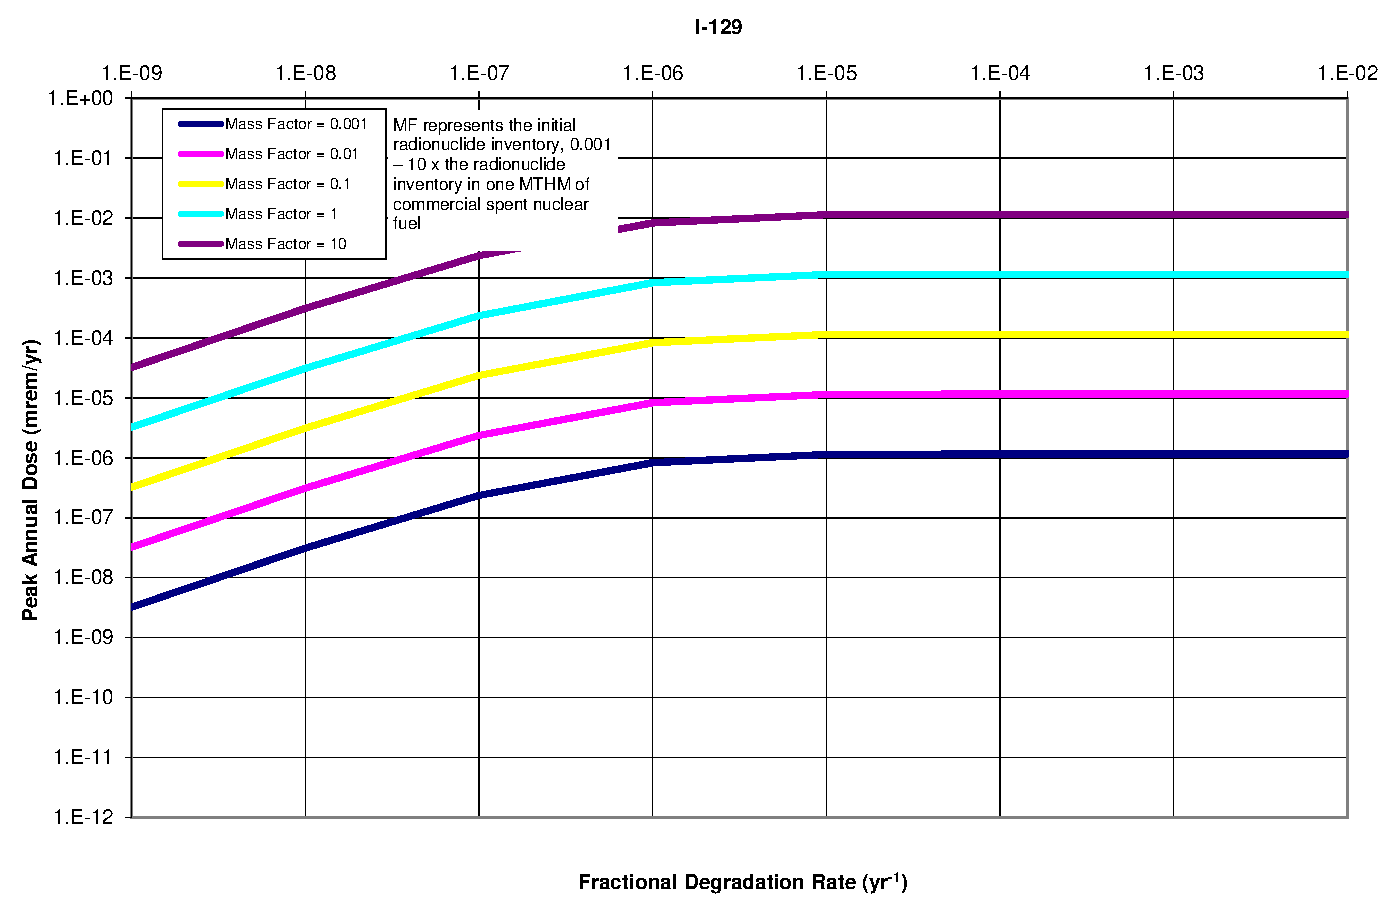
\includegraphics[width=\linewidth]{129IDegRate.eps}
  \caption{$^{129}I$ waste form degradation rate sensitivity.}
  \label{fig:WFDegI129}
\end{figure}
In Figure \ref{fig:WFDegI129}, highly soluble and non-sorbing $^{129}I$ 
demonstrated a direct proportionality between dose rate and fractional 
degradation rate until a turnover where other natural system parameters dampened 
transport.
\end{frame}

\begin{frame}[c]
  \frametitle{Case V : Waste Form Degradation Rate and Inventory}
\begin{figure}[ht!]
  \centering
  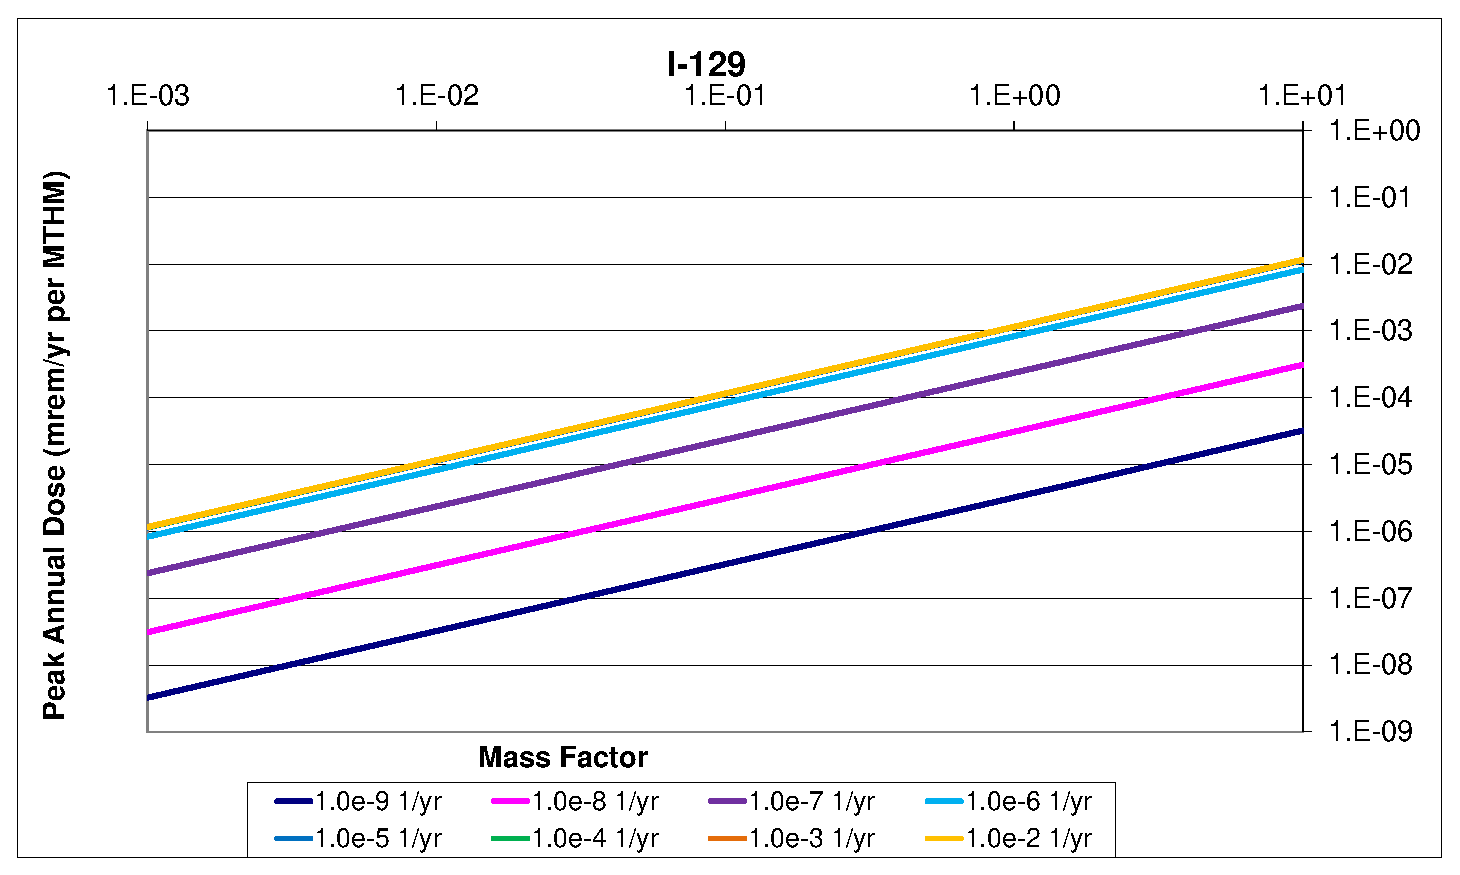
\includegraphics[width=\linewidth]{129IMF.eps}
  \caption{$^{129}I$ inventory multiplier sensitivity.}
  \label{fig:WFDegI129MF}
\end{figure}

It also domonstrated a direct proportionality to the inventory 
multiplier, as seen in Figure \ref{fig:WFDegI129MF}. 
\end{frame}



\begin{frame}[c]
  \frametitle{Case V : Waste Form Degradation Rate and Inventory}
\begin{figure}[ht!]
  \centering
  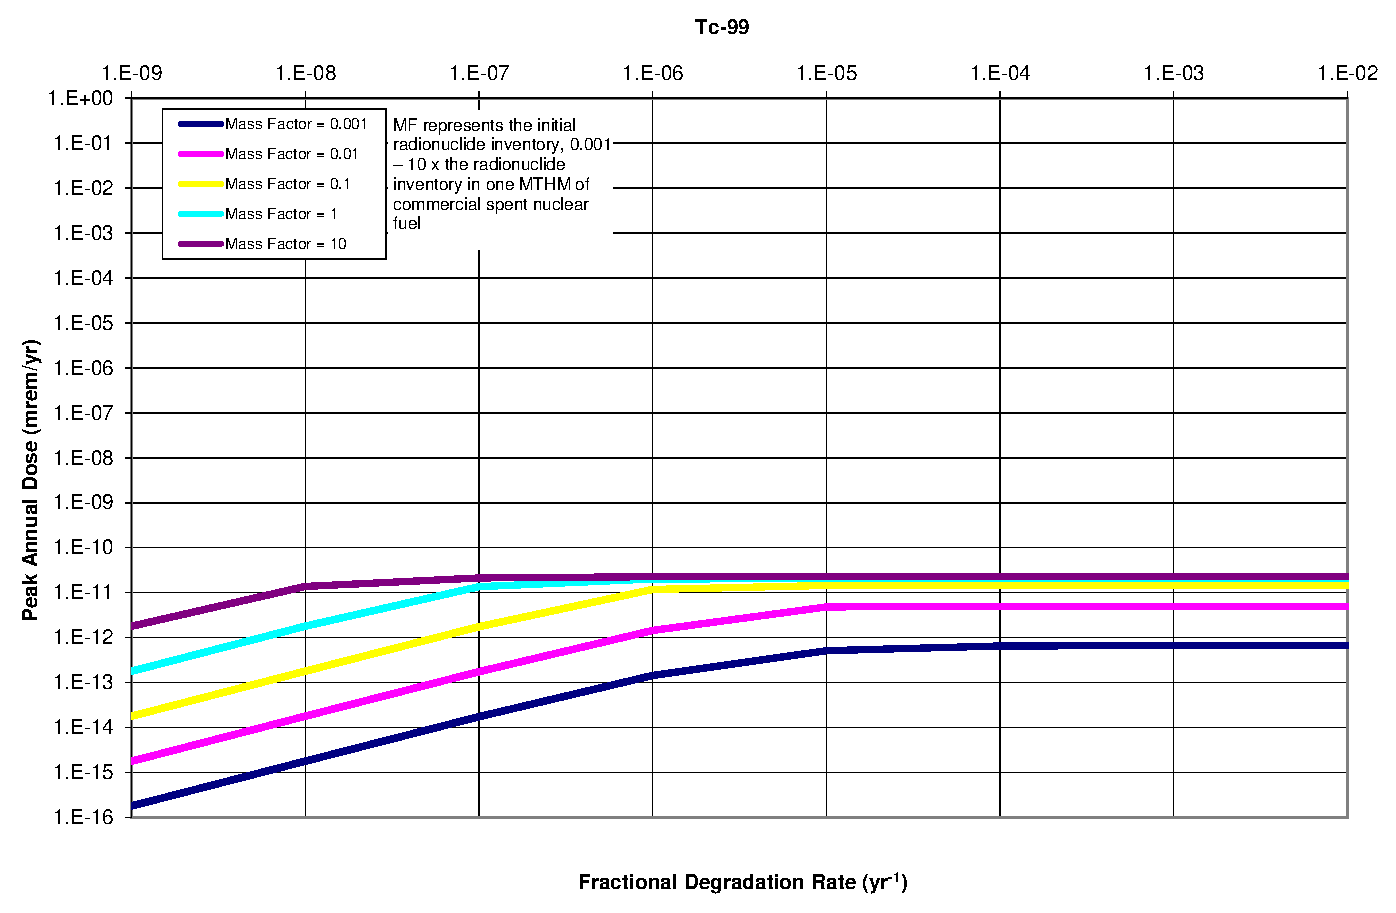
\includegraphics[width=\linewidth]{99TcDegRate.eps}
  \caption{$^{99}Tc$ waste form degradation rate sensitivity.}
  \label{fig:WFDegTc99}
\end{figure}
The peaks for solubility limited, sorbing elements such as $Tc$ and $Np$, on the 
other hand, have a more dramatic turnover.  For very high degradation rates, the 
dependence on mass factor starts to round off due to attenuation by solubility 
limits, as can be seen in Figures 
\ref{fig:WFDegTc99}, and \ref{fig:WFDegTc99MF}.
\end{frame}

\begin{frame}[c]
  \frametitle{Case V : Waste Form Degradation Rate and Inventory}
\begin{figure}[ht!]
  \centering
  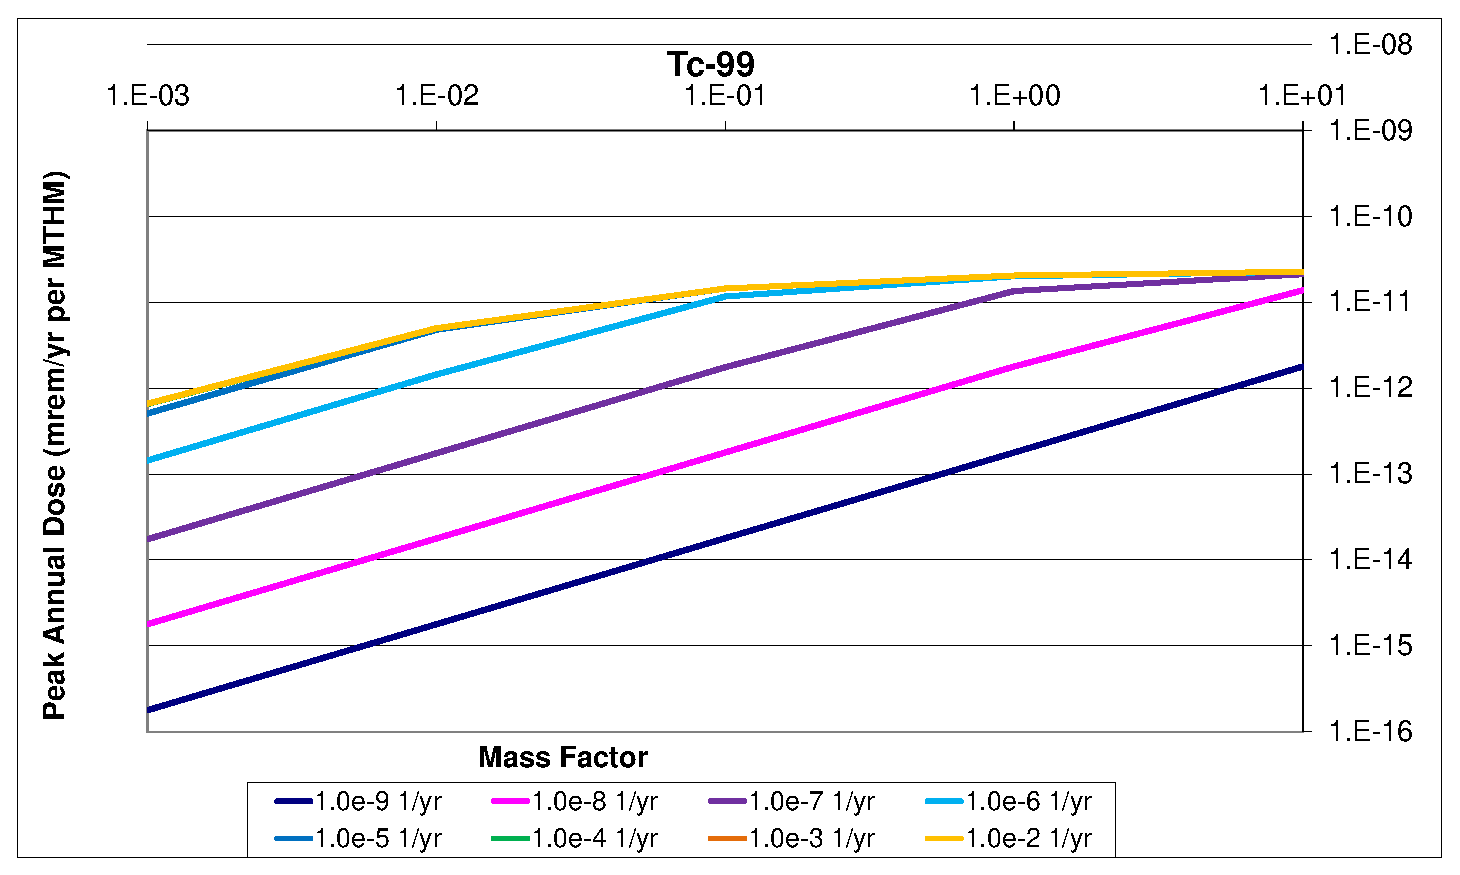
\includegraphics[width=\linewidth]{99TcMF.eps}
  \caption{$^{99}Tc$ inventory multiplier sensitivity.}
  \label{fig:WFDegTc99MF}
\end{figure}
The peaks for solubility limited, sorbing elements such as $Tc$ and $Np$, on the 
other hand, have a more dramatic turnover.  For very high degradation rates, the 
dependence on mass factor starts to round off due to attenuation by solubility 
limits, as can be seen in Figures 
\ref{fig:WFDegTc99}, and \ref{fig:WFDegTc99MF}.
\end{frame}

\begin{frame}[c]
  \frametitle{Case V : Waste Form Degradation Rate and Inventory}
Solubility limited and sorbing isotopes such as $^{99}Tc$ demonstrated a direct 
proportionality to fractional degradation rate until attenuation by their 
solubility limits and other natural system parameters.  
\end{frame}

  

\begin{frame}[c]
  \frametitle{Case V : Waste Form Degradation Rate and Inventory}
  <++>
\end{frame}

\begin{frame}[c]
  \frametitle{Case V : Waste Form Degradation Rate and Inventory}
  <++>
\end{frame}
